\subsubsection{Numerical implementation}

The update functions are given as:
\begin{align}
    \tilde{I}^{m+\frac{1}{2}}_{n+\frac{1}{2}} = \tilde{I}^{m-\frac{1}{2}}_{n+\frac{1}{2}} + \alpha\left(V^{m}_{n} - V^{m}_{n+1}\right) \label{update}, \quad\quad
    V^{m+1}_n = V^{m}_{n} + \alpha\left(\tilde{I}^{m+\frac{1}{2}}_{n-\frac{1}{2}}-\tilde{I}^{m+\frac{1}{2}}_{n+\frac{1}{2}}\right),  
    \end{align}
    
where
\begin{equation}
\alpha \triangleq \frac{v\Delta t}{\Delta z}
    \label{alpha}
\end{equation}

is the dimensionless Courant factor and
\begin{equation}
    \tilde{I}^{m+\frac{1}{2}}_{n+\frac{1}{2}} = I^{m+\frac{1}{2}}_{n+\frac{1}{2}}R_c
    \label{Itil}
\end{equation}
is the rescaled current.

At the boundaries the update function for $V$ takes another form.
\begin{itemize}
    \item At $z = 0$\\
    The voltage update function is given as:
    \begin{equation}
        V^{m+1}_{0} = V^{m}_{0} + \frac{2\Delta t}{C\Delta z}\left(I^{m+\frac{1}{2}}_{g} - I^{m+\frac{1}{2}}_{\frac{1}{2}}\right),
        \label{BC1}
    \end{equation}
    with 
    \begin{equation}
        I^{m+\frac{1}{2}}_{g} = \frac{E^{m+\frac{1}{2}}_{g}}{R_{g}}-\frac{V^{m}_{0}+V^{m+1}_{0}}{2R_g}.
        \label{Ig}
    \end{equation}
    Substituting (\ref{Ig}) in (\ref{BC1}) and using (\ref{alpha}), the two relations $v=\frac{1}{\sqrt{LC}}$ and $R_c=\sqrt{\frac{L}{C}}$ yields, 
    after some rearrangements:
    \begin{equation}
        V^{m+1}_{0} = K_{1}V^{m}_{0} + \kappa_{1}\left(E^{m+\frac{1}{2}}_{g}\frac{R_c}{R_{g}} - \tilde{I}^{m+\frac{1}{2}}_{\frac{1}{2}}\right)
    \end{equation}
    where
    \begin{align}
        K_{1} & = \frac{R_{g}-\alpha R_{c}}{R_{g}+\alpha R_{c}},\\
        \kappa_{1} & = \frac{2\alpha R_{g}}{R_{g}+\alpha R_{c}},
    \end{align}
    are two dimensionless constants named respectively the reflection coefficient and voltage spliiter coefficient.
    \item At $z = d$\\
    
    \begin{center}
    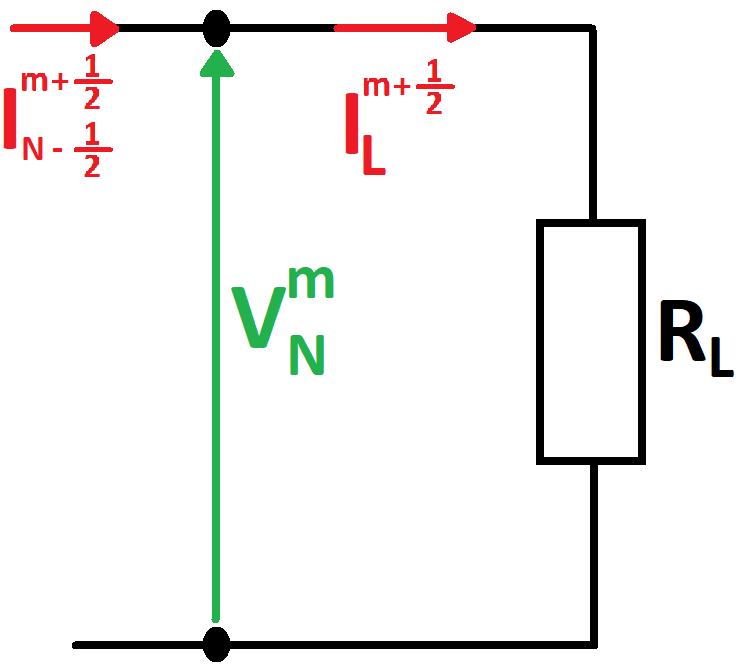
\includegraphics[scale=0.25]{BC2}
    \end{center}

    The voltage update function becomes:
    \begin{equation}
        V^{m+1}_{N} = V^{m}_{N} + \frac{2\Delta t}{C\Delta z}\left(I^{m+\frac{1}{2}}_{N-\frac{1}{2}} - I^{m+\frac{1}{2}}_{L}\right)
        \label{BC2}
    \end{equation}
    Kirchoff's voltage law in discretized form states that
    \begin{align}
        I^{m+\frac{1}{2}}_{L} & = \frac{V^{m+\frac{1}{2}}_{N}}{R_{L}}\\
        & = \frac{V^{m}_{N}+V^{m+1}_{N}}{2R_{L}}
        \label{IL}
    \end{align}
    Subsituting (\ref{IL}) in (\ref{BC2}) and using the same relations as for $z=0$ yields, 
    after some rearrangements:
    \begin{equation}
        V^{m+1}_{N} = K_{2}V^{m}_N + \kappa_{2}\tilde{I}^{m+\frac{1}{2}}_{N-\frac{1}{2}},
    \end{equation}
    where
    \begin{align}
        K_{2} & = \frac{R_{L}-\alpha R_{c}}{R_{L}+\alpha R_{c}},\\
        \kappa_{2} & = \frac{2\alpha R_{L}}{R_{L}+\alpha R_{c}},
    \end{align}
    are two dimensionless constants with the same names as the constants at $z=0$.

\end{itemize}

\subsection{Resistive and capacitive load}

\subsubsection{Numerical implementation}

Now if there would be a capacitor added to the load the following situation will occur
    
\begin{center}
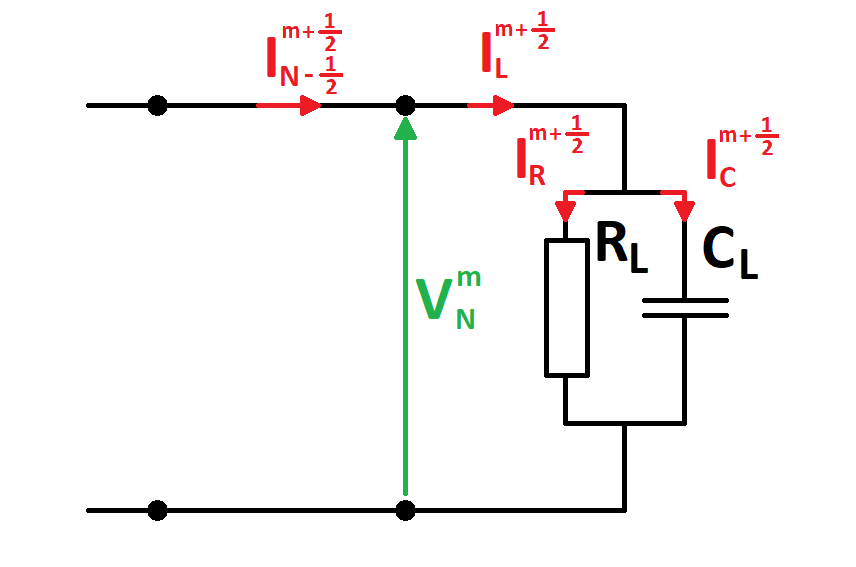
\includegraphics[scale=0.35]{BC2_cap}
\end{center}

Kirchoff's current law states that
\begin{equation}
    I^{m+\frac{1}{2}}_{L} = I^{m+\frac{1}{2}}_{R} + I^{m+\frac{1}{2}}_{C}.
    \label{IL2}
\end{equation}
Using Kirchoff's voltage law at the resistor gives
\begin{align}
    I^{m+\frac{1}{2}}_{R} & = \frac{V^{m+\frac{1}{2}}_{N}}{R_{L}}\\
    & = \frac{V^{m}_{N}+V^{m+1}_{N}}{2R_{L}}
    \label{IR}
\end{align}
The relation between the current and the voltage at the capitor is given as
\begin{equation}
    \hat{i} = C\frac{\partial \hat{v}}{\partial t}.
\end{equation}
For a first order FDM this turns into
\begin{equation}
    I^{m+\frac{1}{2}}_{C} = C_{L}\frac{V^{m+1}_{N} - V^{m}_{N}}{\Delta t}.
    \label{IC}
\end{equation}
Substituting (\ref{IR}) and (\ref{IC}) into (\ref{IL2}) gives
\begin{equation}
    I^{m+\frac{1}{2}}_{L} = \left(\frac{1}{2R_{L}}+\frac{C_{L}}{\Delta t}\right)V^{m+1}_N + \left(\frac{1}{2R_{L}}-\frac{C_{L}}{\Delta t}\right)V^{m}_N
\end{equation}
and can be rewritten as
\begin{equation}
    \tilde{I}^{m+\frac{1}{2}}_{L} = \frac{R_{c}}{2Z_{2}}V^{m+1}_N + \frac{R_{c}}{2Z_{1}}V^{m}_N
    \label{IL2_final}
\end{equation}
with
\begin{align}
    Z_{1} &= \left(\frac{1}{R_{L}}-2\frac{C_{L}}{\Delta t}\right)^{-1} = \frac{R_{L}\Delta t}{\Delta t - 2 C_{L}R_{L}} \nonumber\\
    Z_{2} &= \left(\frac{1}{R_{L}}+2\frac{C_{L}}{\Delta t}\right)^{-1} = \frac{R_{L}\Delta t}{\Delta t + 2 C_{L}R_{L}} \label{eq:Z}
\end{align}
Substituting (\ref{IL2_final}) into the adjusted voltage update function at $z=d$ yields
\begin{equation}
    V^{m+1}_{N} = K'_{2}V^{m}_N + \kappa'_{2}\tilde{I}^{m+\frac{1}{2}}_{N-\frac{1}{2}},
\end{equation}
where
\begin{align}
    K'_{2} & = \frac{Z_{2}}{Z_{1}}\frac{Z_{1}-\alpha R_{c}}{Z_{2}+\alpha R_{c}},\\
    \kappa'_{2} & = \frac{2\alpha Z_{2}}{Z_{2}+\alpha R_{c}}.
\end{align}

\subsubsection{Influence of C}

First thing to notice is that when $C_{L} = 0$ then $K'_{2} = K_{2}$ and $\kappa'_{2} = \kappa_{2}$. This is a good
sign since it stays consistent with the previous update equation.\\
Secondly in relations \ref{eq:Z} there is a time step dependecy, hence the two dimensionless
coefficients in the boundary update function at $z=d$ are also dependent on the implemented time step. Let's consider a
well chosen time step and just look at the effect of changing $C_{L}$.
\begin{itemize}
    \item $C_{L} \rightarrow 0$ :
        $K'_{2} \rightarrow K_{2}$ and $\kappa'_{2} \rightarrow \kappa_{2}$, initial situation
    \item $C_{L} \rightarrow \infty$ :
        $ K'_{2} \rightarrow 1$ and $\kappa'_{2} \rightarrow 0$, fully reflected wave
    \item $C_{L} \rightarrow \frac{\Delta t}{2R_{L}}$ :
        $K'_{2} \rightarrow \frac{Z_{2}}{Z_{2}+\alpha R_{C}}$ and $\kappa'_{2} \rightarrow \frac{2\alpha Z_{2}}{Z_{2}+\alpha R_{C}}$, this shows that the division by zero for $Z_1$ does not lead to any problems.
\end{itemize}

\begin{figure}[H]
    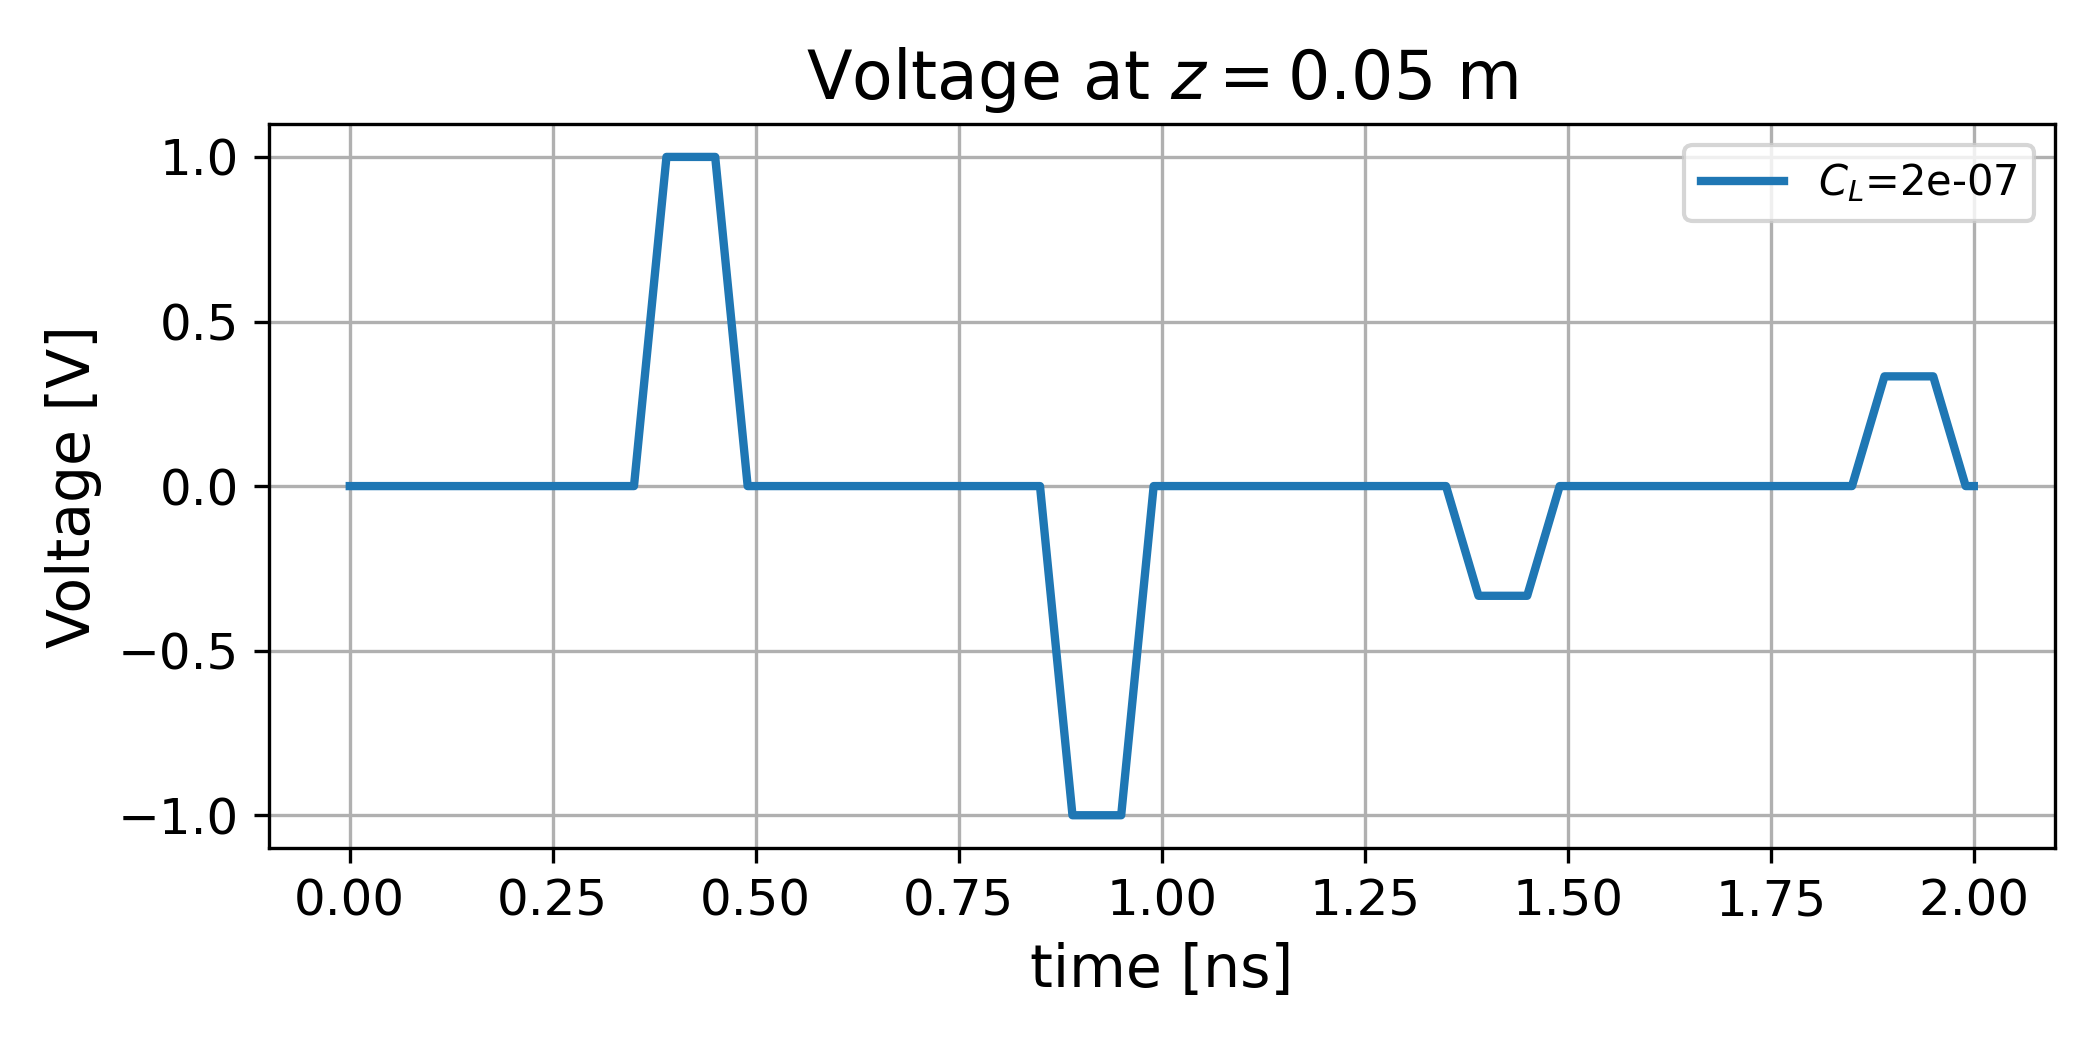
\includegraphics[scale=0.5]{example_C=2e-07_time.png}
    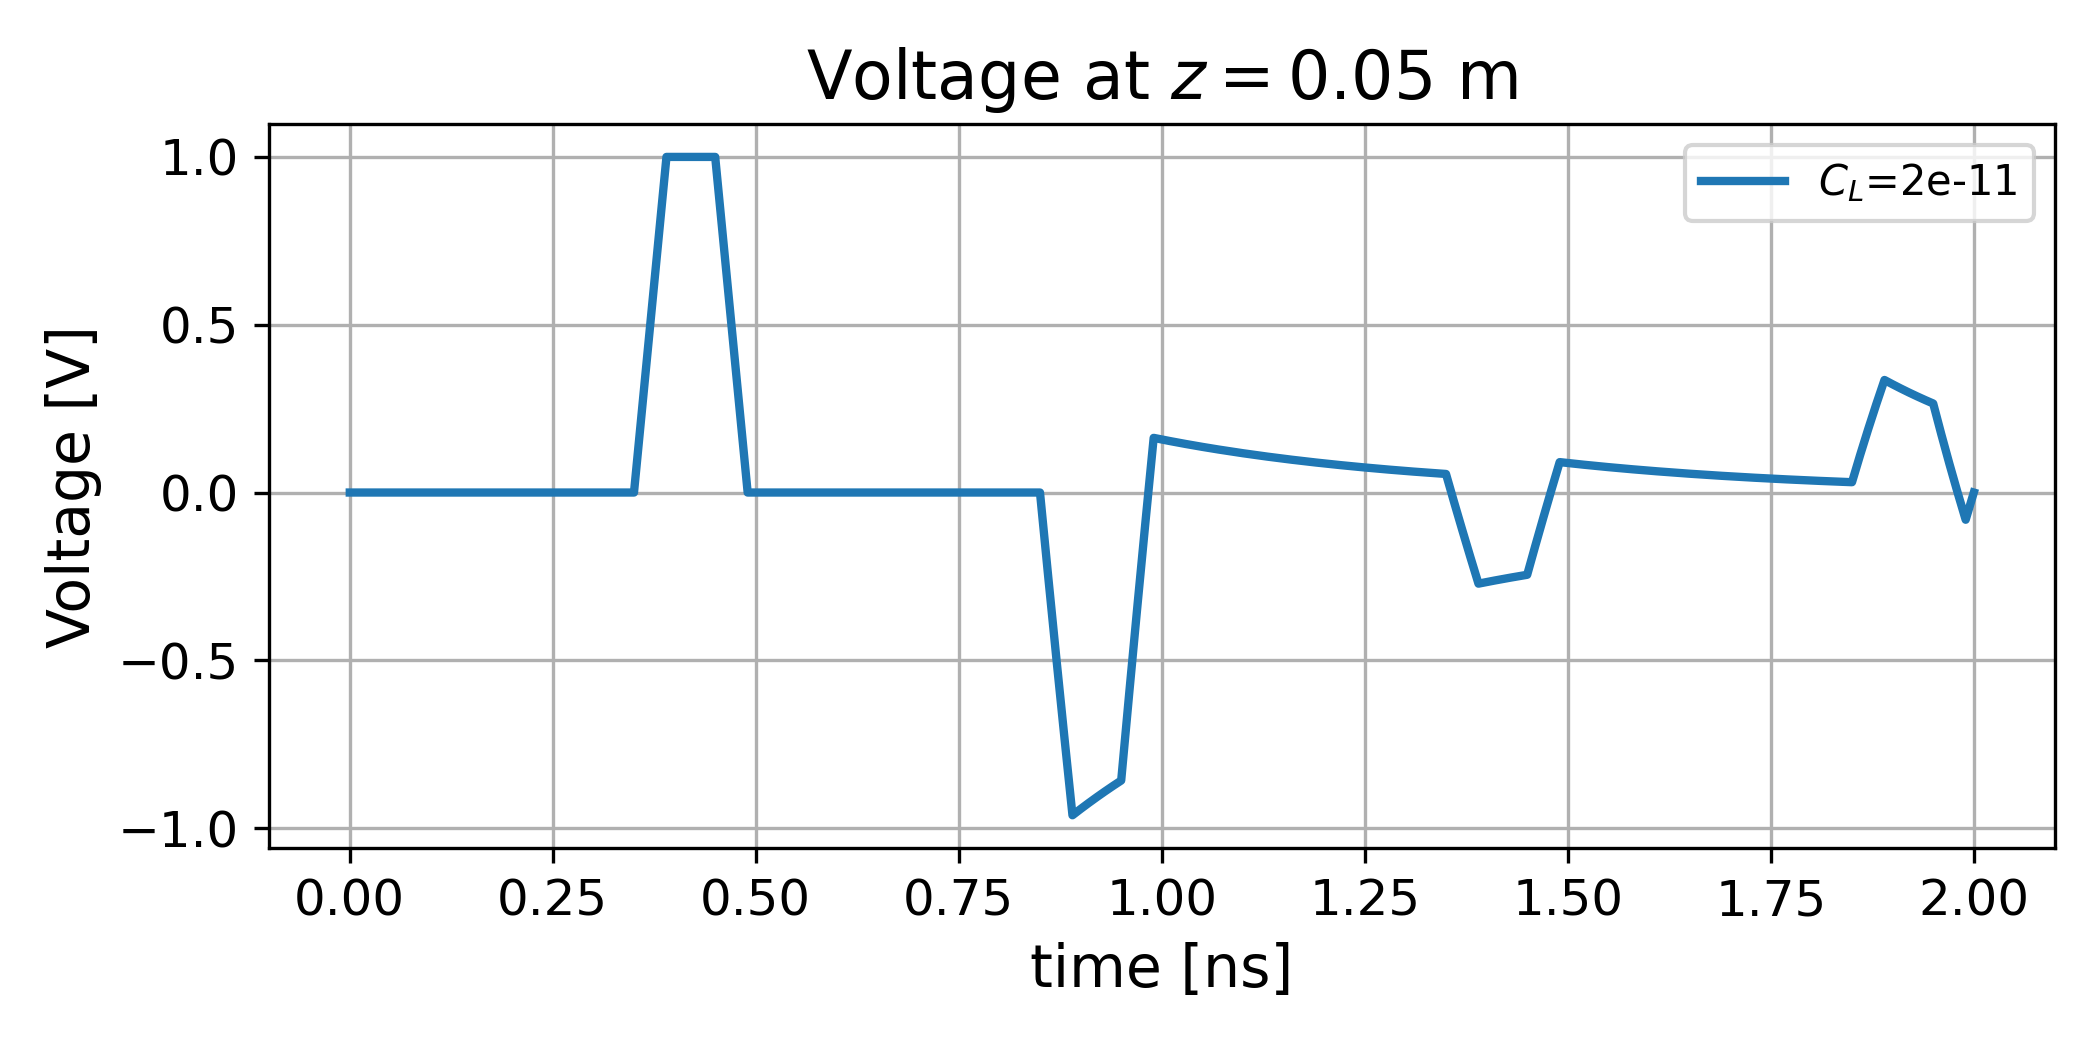
\includegraphics[scale=0.5]{example_C=2e-11_time.png}

    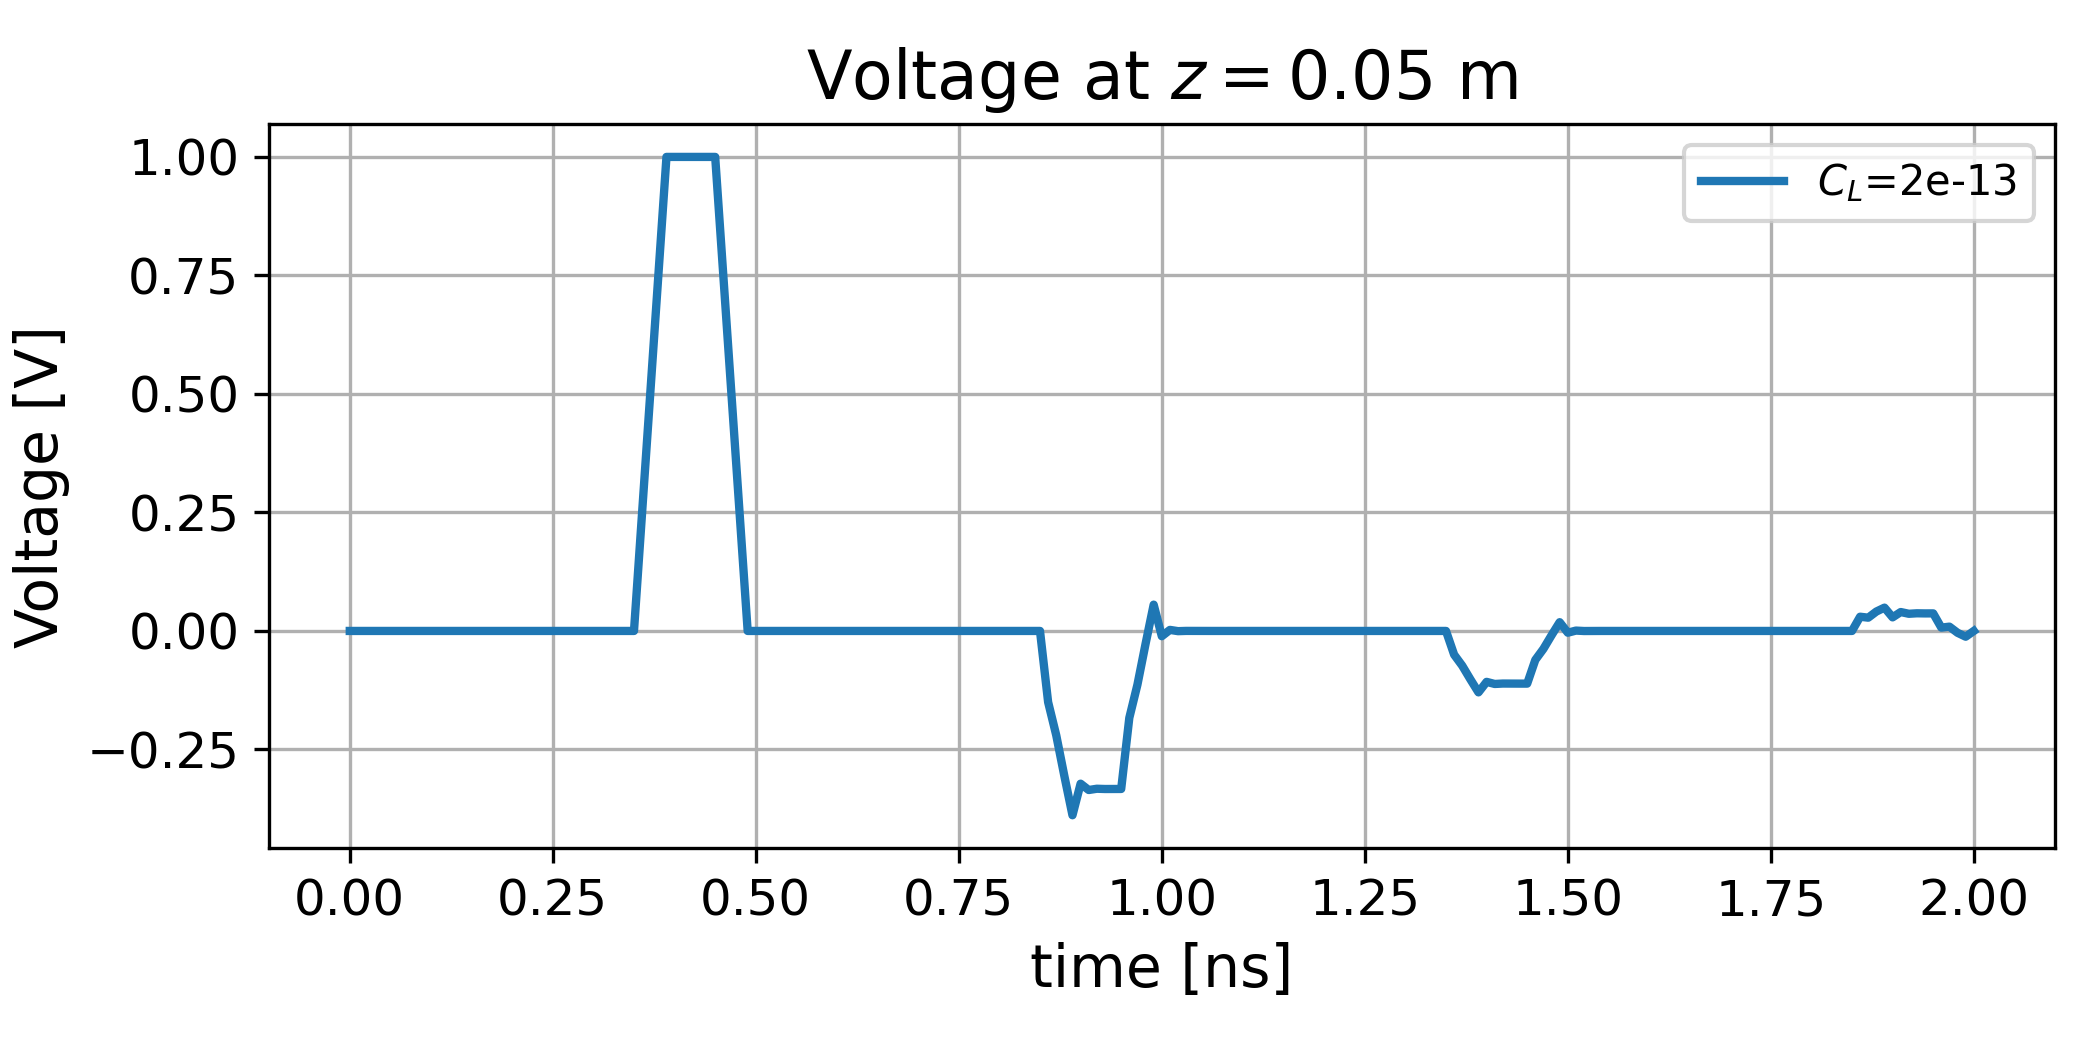
\includegraphics[scale=0.5]{example_C=2e-13_time.png}
    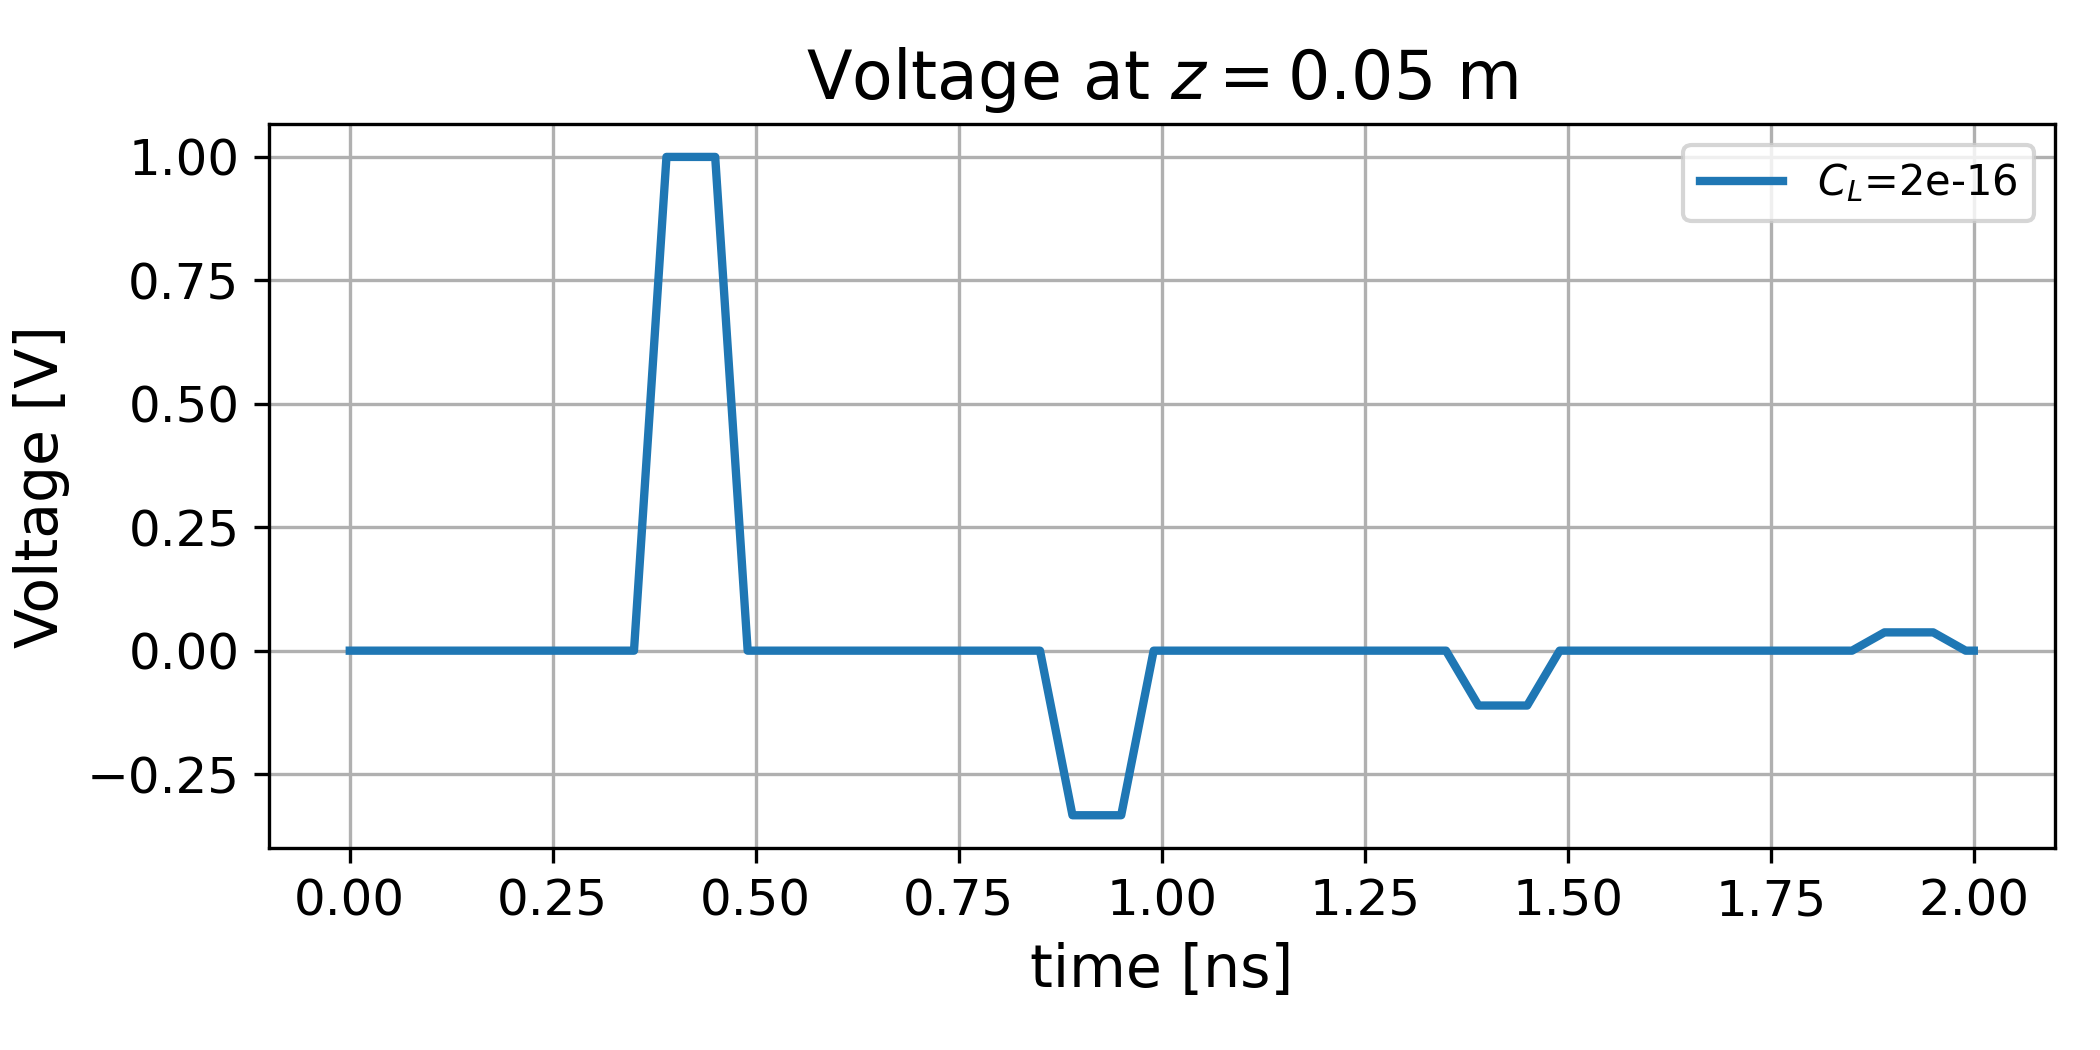
\includegraphics[scale=0.5]{example_C=2e-16_time.png}
    \caption{Different values for the load capacitance}
    \label{fig:effect_CL}
\end{figure}

From figure \ref*{fig:effect_CL} the following obesrvations can be made:
\begin{itemize}
    \item For large values of the capacitance no energy loss will occur at the load, i.e. the amplitude of the voltage does not change when passing the load. The capacitor has enough capacitance to store the whole bit and return it to the transmision line.
    \item For intermediate values for the capacitance, i.e. $C_L = 2e-11$, the decharging of the capacitor can clearly be seen (exponetial drop).
    \item When the capacitance gets very low its effect gets negligible.
\end{itemize}
